%%%%%%%%%%%%%%%%%%%%%%%%%%%%%%%%%%%%%%%%%%%%%%%%%%%%%%%%%%%%%%%%%%%%%%%%%%%%%%%%
% This chapter covers the design aspects, primarily on visual design and
% touch interactions 
%  
% - Should probably talk about active versus inactive versus context objects 
%   in the 3D visualization section
%%%%%%%%%%%%%%%%%%%%%%%%%%%%%%%%%%%%%%%%%%%%%%%%%%%%%%%%%%%%%%%%%%%%%%%%%%%%%%%%
\chapter{Designing Descriptive Non-photorealistic Rendering}
This chapter covers our visual design process and our rationales of our
design decisions. The system interface, as seen in Figure \ref{figure:overview},
is composed of four major components:

\begin{itemize} [noitemsep]
   \item 3D Visualization: The central point of the visualization system
   is a stylized rendering representing the physical entities in the text documents,
   the visualization can be zoomed and rotated to explore different viewing
   perspectives. Each entity is rendered with respect to a function which denotes
   its importance. We explore different rendering styles to take advantage of
   viewers' preattentive perception, allowing them to quickly uncover the
   important information.

   \item Lens Widget: The lens widget is a detail-on-demand tool. It is used
   to specify spatial regions on the \threed visualization. Entities under the
   specified space are considered to be in focus, and more information about
   these entities are shown beside the lens as heatmaps.

   \item Heatmap Widget: The heatmap displays time series data at the lowest
   granularity level in order to provide trend and pattern analysis. It is
   organized into a grid; each cell is shaded in accordance with its score of
   that time period. In addition, the heatmap identifies the entity names and
   their raw numerical scores.
   
  \item Document Widget: The document widget displays the source text documents.
  The panel displays documents relating to the current selected objects and
  applies highlights to all relevant keywords.
\end{itemize}

 
In addition, two domain specific widgets provide filtering functions to
visualize subsets of the text corpus. These widgets are created from the
metadata in the documents, they are:

\begin{itemize} [noitemsep]
  \item Time Filter: The filter is composed of two independent range sliders
  with different granularity: year and month. The filter allows viewers to
  adjust the time range for the visualization. Accompanying each range slider is
  a histogram showing the accumulated volume of complains over a time period.
  The widget itself is place at the top-left of the display space.
  
  \item Hierarchy Filter: The hierarchy filters are placed at the
  top portion of the display similar to a series of drop-down menus or spinners.
  The hierarchy filters allow successive refinement of dataset by means of
  filtering on organizational hierarchies. Going top down, the system supports:
  Vehicle Manufacturer, Vehicle Make, Vehicle Model and Vehicle Year. Hierarchy
  filter is also used to select two different vehicle types when making
  comparisons.
\end{itemize}

 
    % === Figure ===
	\begin{sidewaysfigure}
	 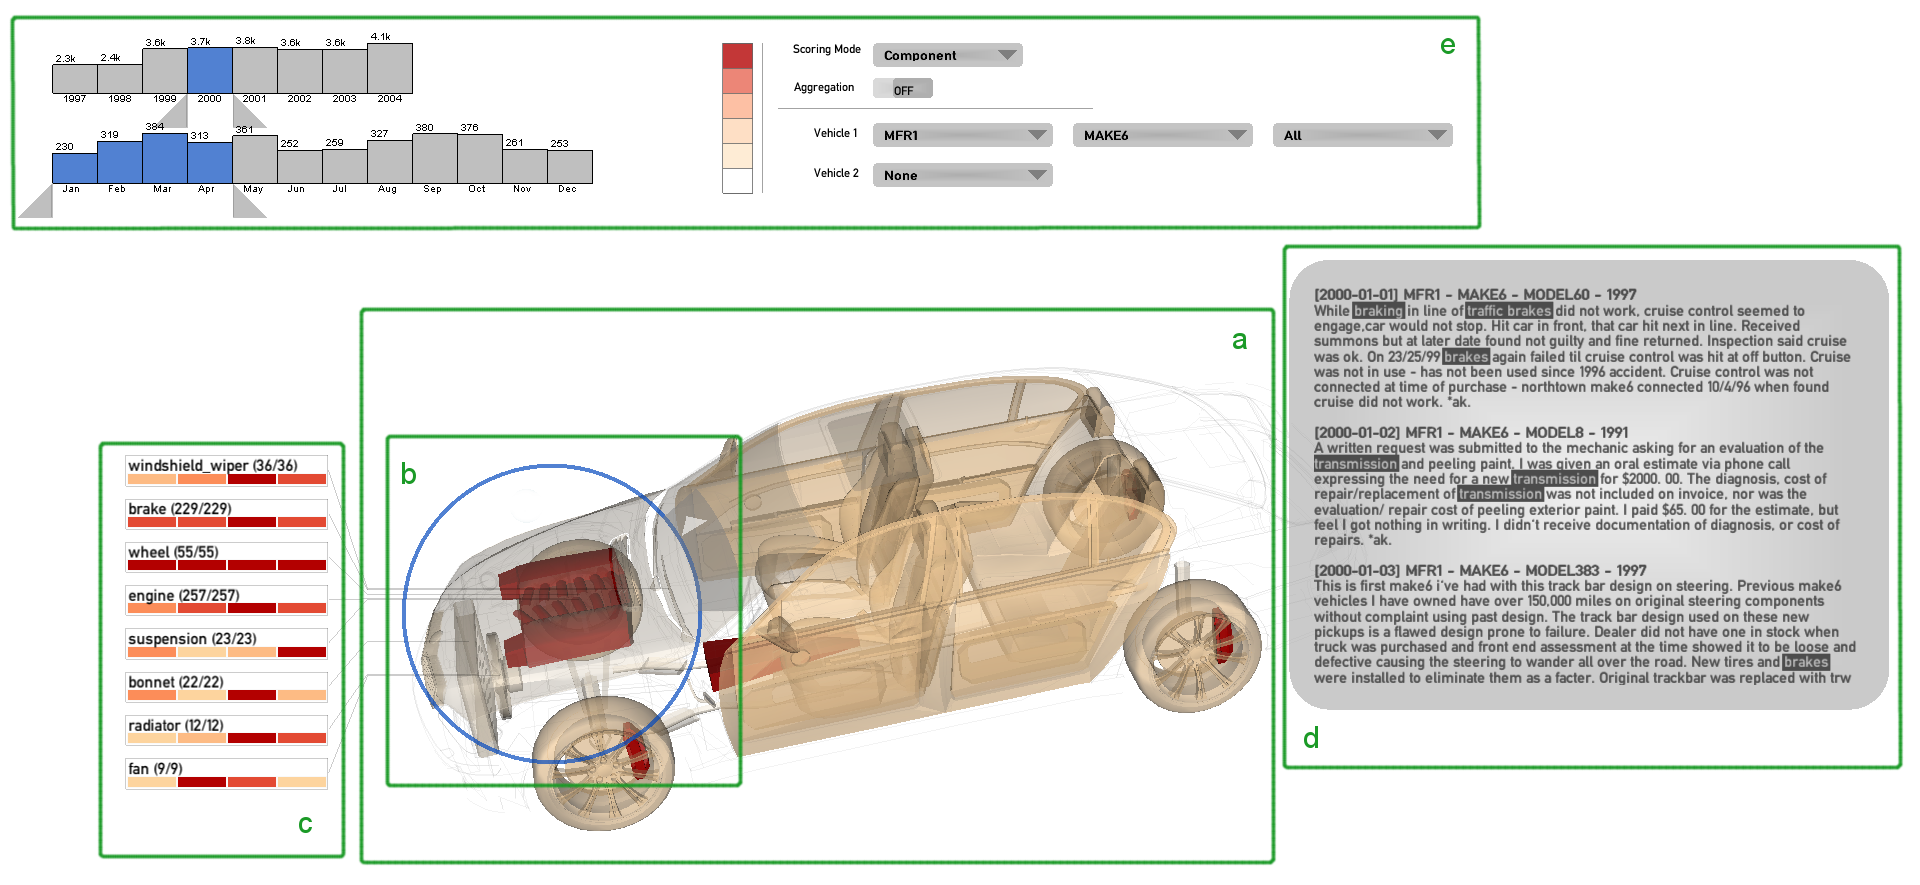
\includegraphics[width=\columnwidth]{overview_2_annotated.png}
	 \centering  
	 \caption[Interface Overview]{System Overview: The 3D visualization (a), lens widget (b), heatmap widget (c), document widget (d), and filters (e). }
	 \label{figure:overview}  
	\end{sidewaysfigure}
	% ==============  

The following subsections will describe each visualization components in
greater detail, with respect to how each widget works and their design trade
offs.


\section{3D Visualization}
This section describes how to perceive the \threed visualization, how it was
designed and discusses various design trade-offs.

\subsection{Rationale}
A major part of our design for this thesis is the mapping of abstract semantics
onto realistic looking, \threed models. But this can also be a source of
complication. We have to deal with the additional difficulties of navigating in
three dimensional space as well as work around perceptual limitations. So why
use \threed models in the first place? Familiarity with the models and varied
exploration methods were key motivations. The familiarity with how the physical
entities look in real life means people do not have to learn additional visual
mappings. Communication may be easier because there is a shared common ground
among the different parties involved. Proximal relationships are also easily
perceived if they have realistic spatial mappings and can encourage more
thorough exploration of the dataset. These advantages are not readily present in
abstract representations, while with careful design it is possible to overcome
many of the pitfalls of perceiving \threed graphics. Lastly, we are not merely
mimicking \threed objects, our visualization goes further to facilitate user
oriented tasks~\cite{Shneiderman2003}. We enhanced the rendering process with
NPR techniques, along with interactions to explore the \threed space in an intuitive manner. 

Yet another argument is that the use of a set of \twod images can also convey
realism, our opinion is that they lack the expressive power and playfulness of a
fully rendered \threed model. Flat image representation would likely result in
multiple images, used to cover different viewing perspectives, this can result
in more cognitive load due to viewers having to switch between images to
see different data.


\subsection{Visual Mapping}
Because our visualization environment makes use of 3 dimensional space,
extra care are taken into account for the selection of visual variables. Not all 
visual variables are appropriate, shape, position and orientation are inherently
used to represent the geometries on the virtual model, a double encoding of these
variables is likely going to lead to confusion, compromising the ability to
interpret the visualization, or destroy any resemblance of the virtual model to
its real world counterpart. Thus these are rejected in the early part of our
design. Size is an interesting one, in theory size can support most of the
characteristics. However it is implied that all the objects of the same value have the equal size, 
which is certainly not the case for physical objects with sub components. Colour 
and value variables are not used to represent the virtual model, in the sense that 
they are not a part of the  basic geometry building blocks of vertices, line-segments 
and polygons. We found colour and value to be appropriate for our visualization, 
while they do not provide a sense of quantitative measure, the capability to see order, 
selective and associative characteristics makes them a logical choice for an
overview visualization.

Lastly, textures present an interesting option, textures can carry additional 
characteristics, particularly descriptive attributes. It may be possible to use 
textures to simulate certain effects, for example a rusty surface. Nonetheless,
textures do not possess order or quantifiable characteristics and was not
included in our design. However it may be interesting to use textures for
visualizing individual document, we leave this idea as future work.

\subsection{Stylized Rendering}
In order to enhance the message carrying capacity of the visualization, we
considered several NPR techniques as a medium to create  more expressive
illustrations. We associate the entity score with either a NPR technique, or use
the score as a parameter into a NPR function. In accordance with our
requirement, the encoding scheme should be clear and distinguishable by visual
examination(R1) while maintaining the real world aspects. Our effects include
varying stroke, halo/glow, colour variations, and transparency effects.

We chose colour mappings as our primary visual encoding which denotes the
strength of non-zero score entities, and use other techniques to denote
selection and overall context.

Designing a colour scheme for the encoding of the virtual component objects
presented several design trade-offs. We colour each object by mapping its score 
to a linear diverging yellow-orange-red hue scale, which is further divided into 
six discrete scoring bins. While this setup has a limited granularity, it is
easier to perceive a small number of discrete colours than viewing a continuous
scale. We mitigate any ambiguities that may arise with the discrete scale by
providing numerical values with the lens and heatmap widget, which we discuss
further down.


\threed geometries may not be visible due to occlusion or containment.
The first case can be partially solved by altering
the viewing distance and viewing perspective on the visualization, whereas in
the second case no amount of viewing adjustment will solve the occlusion issue.
To address this problem, we double encoded the score as both the
colour and transparency values. The transparency value of each geometric object
is proportional to the entity�s score, such that the higher scored entities
appear more opaque, while the lower scored entities appear more transparent. The
maximum and minimum transparency values are capped between 0.4 and 0.8 such that
no objects are completely opaque or completely transparent. Our transparency scale
is slightly weighted to give more emphasis for more frequently occurring
entities. One challenge of rendering translucent geometries in \threed space is
that the ordering of geometries becomes important for alpha-blending to work
correctly; out-of-sequence geometries can lose their depth cues when blended
together. We discuss this effect, and solutions in further detail in the
implementation chapter.


The zero score has a special semantic in the visualization. When an entity's
score is zero, this indicates that there are no known references of the entity
in the documents. Not rendering them would reduce visual clutter, but comes at a
cost of not having a background reference, which gives visual cues to not only
what viewers are looking at, but also the placement and relative position among
other entity objects. To show that these components are semantically different
than others, the system renders them with silhouette styled edges in a just
noticeable colour so they are visible but not overly
distracting~\cite{BAR2007a}. It is worth noting that 0 scored objects only
provides graphical context, they do not partake in any user interactions.



 

\subsection{Selection}
Selection of entities is used to refine the visualization scope, for example
selecting the windows entity tells the system to only visualize documents that
refer to windows. The system provides several methods for selecting entities,
selections can be made by directly interacting with the \threed visualization,
or through interaction with the heatmap widget.

    % === Figure ===
 	\begin{figure}
 	 \centering  
 	 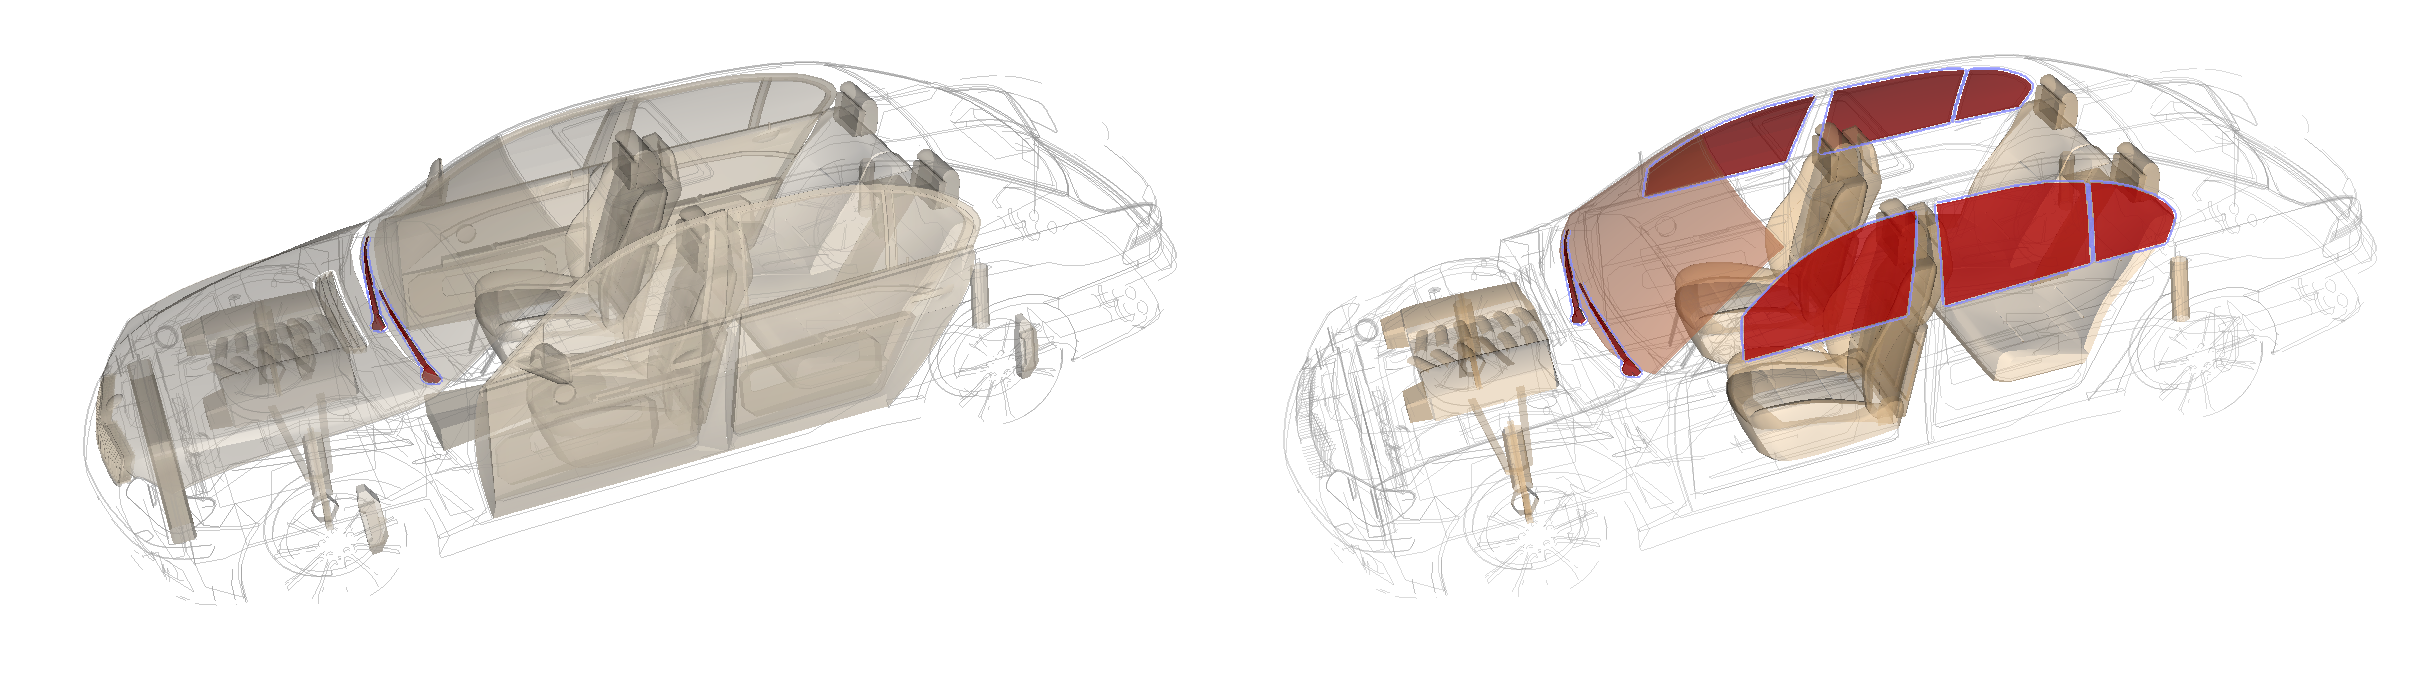
\includegraphics[width=\columnwidth]{select.png}
 	 \caption[Interactive Selection]{The visualization changes to reflect
 	 co-occurrence relations. Left: showing co-occurrences with respect to
 	 windshield wiper. Right: showing co-occurrences with respect to both
 	 windshield wiper and window entities.}
 	 \label{figure:selection}
 	\end{figure}
 	% ==============

By default the application has no entities selected, thus the visualization
reflects the absolute number of occurrences of each entity. As
selections are made, each entity�s score is recomputed to show co-occurrence
relations with the selection, note since selected objects
fully co-occurs with themselves, they are promoted to the highest bin.
In this manner, high correlations are red and highly opaque, while low
correlations are yellow and highly transparent. For example, if a person selects
the windshield wiper, the visualization is rerendered to show entities
that co-occur with the wiper component and the strength of this
relation. If the same person then selects the windows, the visualization
will show co-occurring relation to both windshield wiper and windows. This example
is reflected in Figure \ref{figure:selection}. The rerendering process is
facilitated by an animated transition that interpolates the graphical effects.


% Entity objects can be acquired in two ways: One can directly select the entity
% by performing the tap gesture on the \threed representation, or tapping the
% heatmap through the lens widget. In the case where objects occlude each other
% in \threed space, direct selection will return the object that is closest to
% viewing point. In order to select occluded objects, the scene can be
% rotated to reveal hidden entities. Alternatively, we can use the lens� depth
% functionality to cut away occluding geometries, or directly clicking on the
% heatmap representations which are always available.
% 
%     % === Figure ===
% 	\begin{figure}
% 	 \centering  
% 	 \includegraphics[width=\columnwidth]{interaction_select.png}
% 	 \caption[Interactive Selection]{The visualization changes based on the
% 	 currently selected entities.}
% 	 \label{figure:selection}
% 	\end{figure}
% 	% ==============
% 
% Selection is toggle based. When an entity is selected, we apply a blue borderb
% to the associated heatmap and the line segments that links the heatmap back to
% the visualization. To visually accentuate the selection in \threed
% space, we employ a halo like effect around the hull of the mesh objects. Both
% selection and deselection of any entity triggers an event to recalculate the
% entity scores, an animated sequence then starts to interpolate the colour of
% each \threed object to reflect the scoring change.
% 
% The re-evaluation of the entity scores are based on current selection,
% specifically they are recalculated based on their co-occurrence relation with
% the current selection. Thus, highly co-occurring entities will score higher and
% be more visible than lowly co-occurring entities.
% 
% Selection of an entity with zero score is considered invalid, instead, the
% system will propagate the selection event through the zero scored entities.
 
%\daniel{Stopping here\ldots}

\subsection{Trade-offs}
We recognize that blending different hues in \threed space does not necessarily
produce a result which preserves the original hues, and can potentially lead to
distracting visual artifacts. Different hue preservation schemes
exist~\cite{Chuang2009} but were not implemented for this prototype due to the
added performance complexity (Hue adjustments are done at per pixel level). Subjectively, 
we did not find any visual distractors and thus decided that this was not necessary. A 
single-hue scheme with varying saturation and opacity was tried as well, but we
found it less eye-pleasing and lacks the \emph{pop-out} effect that is more prominent on multi-hue 
colour schemes. 


%Due to known issues with blending, we have tried to use a single hue grey scale 
%with varying brightness, but we found that it was somewhat difficult to distinguish 
%overlapping or contained objects. Subjectively speaking, single-hue also looks
%less aesthetically pleasing, the entities did not have the ``pop-out'' effect
%as we seen with multi-hue schemes. Thus we decided that using  a multi-hue
%scheme was more appropriate, despite the potential blending artifacts.

A second design trade-off was whether lighting effects should be used. Lighting
effects such as specular lighting can create distractions because it can create 
highlights in places of little or no significance. Without any realistic
or simulated lighting effects, the visible colour of the components exactly
matches the colour assigned to the score and as seen on the legend.
However, without any sort of lighting, particularly some type of diffuse lighting, 
the \threed nature of the model, and the details of various components are not
sufficiently visible. Adjacent objects that share the same score appear to be glued together 
as a single component, adding boundary outlines helps but creates undesirable
visual clutters. When lighting effects are enabled, the objects are easily
distinguishable as lighting provides a clear silhouette. However, this type of lighting modifies 
the colour based on the incidence angle of the light rays, thus it no longer matches 
the assigned colour. Ultimately, we decided that the benefits of objects recognition and
familiarity outweigh the colour offsets. The results of our design choices can be seen in
Figure \ref{figure:visualEncoding}.

%Ultimately our design decision is that object recognition and 
%familiarity is important to us. Thus, by restricting the number of hues (6 buckets) 
%and using soft white light, we contend that the lighting effects do not disturb 
%the colour perception enough to obscure which hue-bin the component belongs to. 
%We made the design decision that the benefits of enabling lighting to visually 
%resolve the components outweighed the negative effect of shifting colours away 
%from those displayed in the onscreen legend. The results of our design choices
%can be seen in Figure \ref{figure:visualEncoding}.
 

    % ===== Figure =====
	\begin{figure}
	   \centering  
	   \includegraphics[width=\columnwidth]{visual_encoding.png}
	   \caption[Trade-offs]{Showing the visual design trade offs. Top left: single
	   hue with flat shading. Top right: multi-hue with flat shading. Bottom left: single
	   hue with lighting effects. Bottom right: multi-hue with lighting effects.}
	   \label{figure:visualEncoding}
	\end{figure} 
	% ==================


Since the system visualizes \threed geometry, it can be
tempting to apply other types of techniques. For example we attempted to encode the importance and other 
numerical semantics into a geometrical distortion function that can be applied
directly onto a \threed mesh. In practice, this does not work well for visual evaluation:
in general, objects are of different shapes and sizes, applying a small distortion 
is not entirely obvious while a large distortion can destroy the familiarity of 
the form. It is also more difficult to recognize objects under distortion and to 
compare the degree of distortion among objects.


%Yet another problem is that it is not possible to order or quantify by 
%shape \cite{BER1983a}, which makes the distortion a qualitative measure instead
%of a quantitative one. In addition, the ability to read quantitative value from a 
%distortion field presumes that the viewer has a mental model of what the object 
%looks like without any distortions, an assumption that we cannot make with our 
%intended audiences.  However distortion remains an interesting possibility because 
%we may use distortion to visually paint the action words, testing this will be 
%part of our future work.




\section{Lens Widget} 
Using a metaphor of looking through a magnifying glass to reveal better details
about a specific subject, we created an interactive lens widget to extract and
show detailed information about entities in the text documents. With respect to the information
seeking process, this approach combines both filter and detail-on-demand phases.

The lens widget operates in a hybrid \twod/\threed space, the lens itself exists
on a flat \twod plane, it casts a cylindrical querying volume into the scene.
When the lens is positioned over the visualization, each entity object is tested to see if their
corresponding meshes are in the lens' querying volume. We use the centroid to do the inclusion
test, though more accurate, albeit slower methods exist using
image based algorithms~\cite{Ali2005}. Entities that are under the lens' area of
focus have detailed information, shown as heatmaps on the left and right side of
the lens widget. Connecting line segments are drawn from entities to their
heatmaps to show association: first the heatmap is connected back to the lens'
circumference, then from the circumference back to the entity's projected centroid.


    % ===== Figure =====
	\begin{figure}
	 \centering  
	 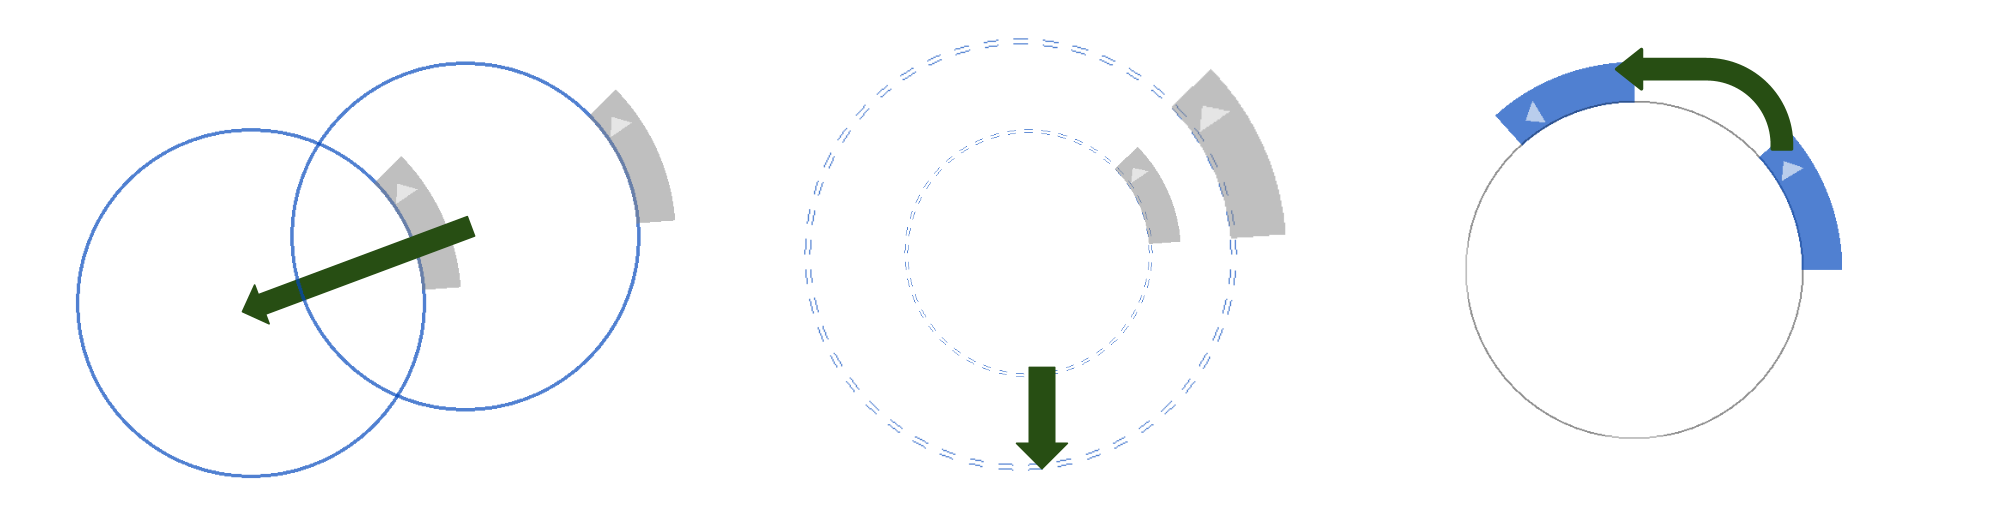
\includegraphics[width=\columnwidth]{lens_interaction.png}
	 \caption[Lens Interaction]{Interactions, from left to right: moving the
	 lens, resizing the lens and adjusting the depth handle.}
	 \label{figure:lens_interaction}
	\end{figure}
	% ==================


    % ===== Figure =====
	\begin{figure}
	 \centering  
	 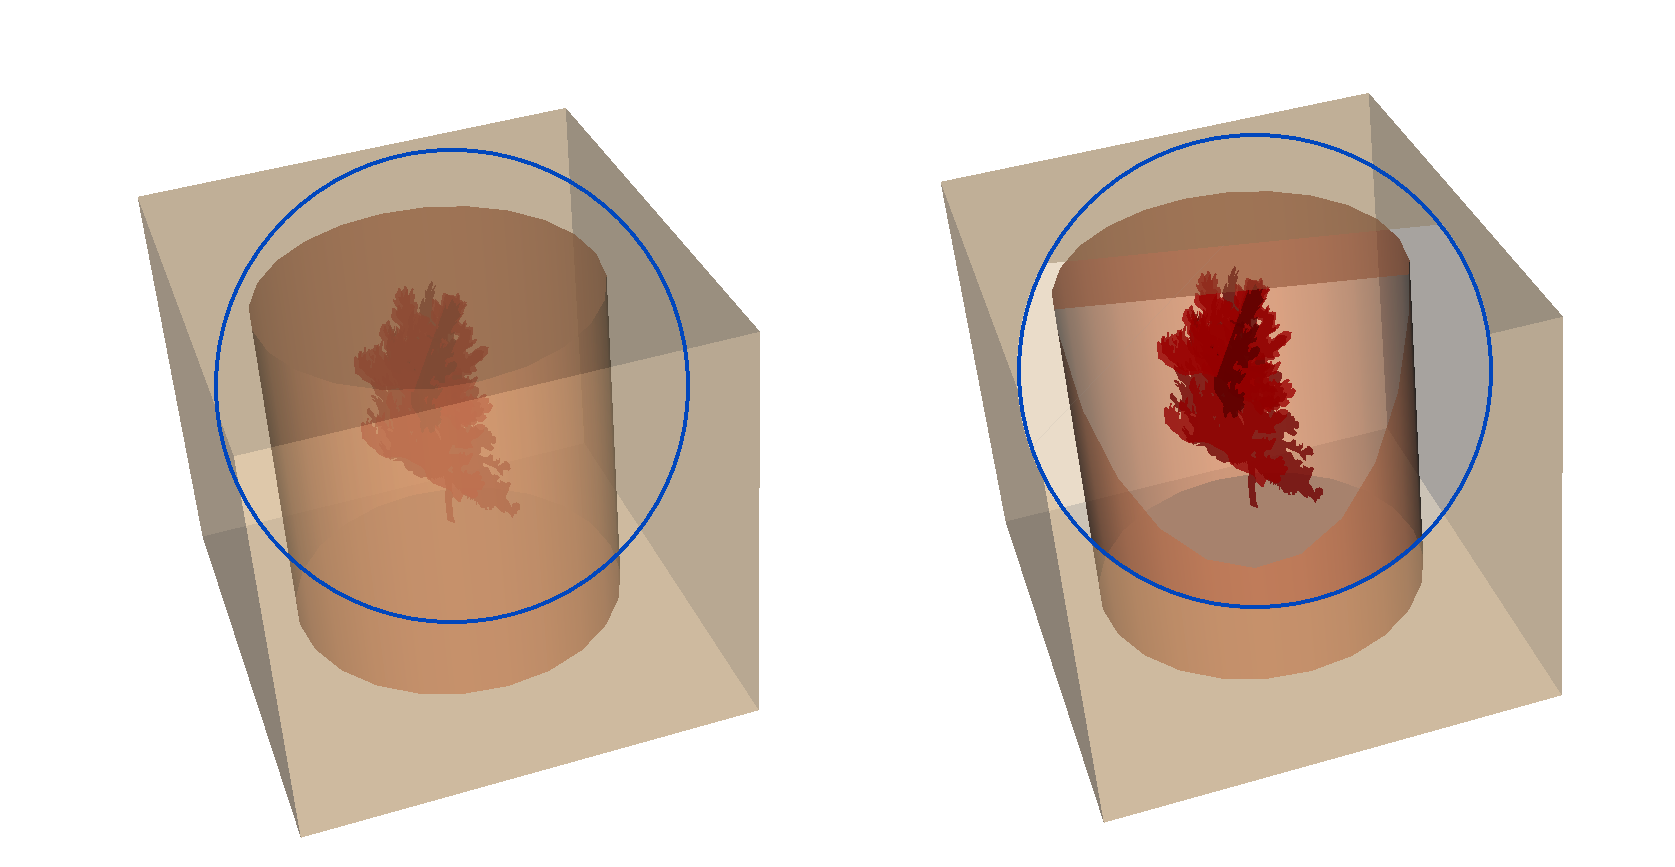
\includegraphics[width=\columnwidth]{lens_example.png}
	 \caption[Lens Depth]{The lens widget can be tuned to expose
	 occluded geometries. Left shows the unaltered geometry. On the right, the
	 lens cuts into the geometric shapes to expose the tree contained in the
	 cylinder, which itself is contained in a box.}
	 \label{figure:lens_depth}
	\end{figure}
	% ==================
	
	
The lens widget utilizes its own rendering pipeline, object geometries
are sent into the pipeline as normal, rendering results are 
then stored in an intermediate buffer and later combined in fragment
shaders with the default scene. This is an independent
process, and thus allows us to render the lens� scene with a different rendering
style and semantic. To visualize the lens widget itself, we
draw a semi-transparent border around its circumference so viewers
are aware of its existence. When interacting with the lens widget, the
widget becomes active and the system renders the border blue, otherwise 
the default grey colour is used. The semantics of the lens is not impacted by
whether the lens is active or inactive.	



The lens enables three different actions, seen in Figure
\ref{figure:lens_interaction}. The position of the lens can be moved by dragging
within the lens, impacting the currently focused entities and the heatmap charts. The lens can be resized by
dragging on the border of the lens, increasing or decreasing the query
area. Lastly, the depth plane can be adjusted by rotating the depth
selector tab around the circumference of the lens (see Figure
\ref{figure:lens_depth}). The depth plane function provides a method for people
to reduce occlusion, as all entities that are the cut by the plane are drawn in
an outline style, allowing viewers to see through them and into the object. Objects that
are cut off are excluded from any scoring calculations, they also have
their heatmaps hidden to reduce visual clutter. These three interactions
can be combined together to create a rich, flexible query mechanism.


Multiple lens widget are allowed for simultaneous exploration of
different parts of the visualization. For example, if the subject matter is of
an elongated shape, it is possible to use two lens to explore the entities
positioned at either end. However, no semantics are currently defined for
multiple lens to co-exist in the same spatial location, that is, the lens widget
has no defined behaviour when it is overlapped with another lens.


\subsection{Spatial Interaction}
Traditional systems use explicit queries as a mean to
communicate with the underlying data. While this works well for task analysis,
it has an implicit assumption that the person knows something about how the
system works, and how the data is structured. Thus it can be a limiting factor
that prevents a wider audience from using applications without prior training.

In this thesis we take a different approach, the lens widget allows people to
demand and filter detailed information by means of a visual query. Unlike explicit queries,
visual query is done more passively by moving the lens widget about the 
visualization, points of interests, if any, are shown as heatmap charts without
explicit requests. Thus a user is free to roam about the visualization without 
any specific goals or prior knowledge about the data, making the visualization
more playful and open to unexpected discoveries.

%\daniel{Maybe cite the bohemain bookshelf would be appropriate here}


In addition to the freedom of exploration, the lens has an additional 
benefit of allowing people to specify logical regions. Imagine the case where 
a person is asked to investigate issues relating to the ``front'' of the 
vehicle, this query is difficult to formulate, components situated at the front 
need to be identified (which inconvenience  a person with novice expertise), 
and ``front'' itself may be subjective depending on person. By repositioning 
and resizing the lens, a person can identify the front, back, or any other
logical region quite easily.




\section{Heatmap Widget}
The heatmap is an interactive widget that shows entity specific information over
the selected time frame. Each heatmap is designed to communicate how the volume
of complaints changed over time for individual entity components by fitting a
time series data onto a two dimensional grid. In this system, the heatmaps
allows year-to-year and month-to-month comparisons.

% Prior to our heatmap implentation, we have also considered using a simple 
% scatter-plot approach, with time on the X-axis and the volume of complaints on
% the Y-axis. While this solution is simpler to read and likely easier to detect
% long term trend, its major drawback is that it is likely more difficult to
% make seasonal comparisons. For example, imagine a case where we want to compare
% summer to fall over a 4 year span, one must constantly make the context switch
% to decipher which parts of the graph represents summer, and which parts
% represent winter. Also, in extreme cases scrolling need to be utilized for very
% long time frames.

The time segments are arranged chronologically onto a grid like a calendar,
the months are arranged left-to-right in ascending order, and the years arranged 
top-to-bottom in ascending order. The dimension of the heatmap's grid corresponds to 
the selected time on the time widget. Each cell then represents the entity score for
the particular month. We use the same 6-bin colour encoding for the heatmap
widget to keep a consistent colouring scheme throughout the system. The heatmap
label, placed at the top of the widget, shows the entity name, co-occurrence score 
and occurrence score. Note the choice of the entity name is the first word in the 
keyword's synset, which may differ from the actual text.

When examining the heatmap, trends and outliers can be detected visually. The
grid-like view aligns both month and year spatially, allowing viewers to
make yearly (row-to-row) and monthly (column-to-column) comparisons with relative
ease. Two types of interactions are supported by the heatmap widget. Selecting the 
heatmap is equivalent to a selection on the \threed visualization. Performing a hold
over an individual cell toggles a tooltip that displays the numerical score for that
cell, a blue border is drawn around the cell, the same border is linked over all cells
of the same month across visible heatmaps, allowing for quick comparison.


\subsection{Layout}
With respect to heatmaps placement, we have considered two
types of layout around the lens widget: A flush-left/flush-right layout
that places the heatmaps on either left or right side of the lens, and a radial
layout where each heatmap is placed around the lens� circumference. The radial
layout is eye-pleasing, but is unstable during movement transition due to a
single anchor point in the centre, and it is harder to compare across heatmaps
because they are not spatially aligned, thus it was deemed unsuitable. 

For the flush layout, we first sort the object centroids by their 
Y-coordinates in screen space, then we place the heatmaps on
left/right side based on the heuristics below: 
\begin{itemize}[noitemsep]
  \item Heatmap placement should always be outside of the axis-aligned bounding box of the \threed model.
  \item If the entity centroid is closer to the right edge of the bounding box, it will be placed on the right, else left.
  \item If the heatmaps are off the screen space, perform contraction to move it back into screen space.
\end{itemize} 
Since there is no reliance on the centre of the lens for placement, movement of the lens widget will not cause
drastic changes to and thus is more stable when moving the lens over the visualization.

Due to limited display space, not all heatmap are shown at once. A scrolling mechanism, shown
as up and down arrows on the lens, are used to scroll through unseen entity objects, numerical
indicators on each arrow provide a summary of how many entities are hidden in either direction.
We set the maximum visible heatmaps to 8 in this system.
 

\section{Document Widget}
The document widget is the final stage of our drill-down process by providing links 
to the raw text(R4). Each document is divided into two sections,
the header section shows each document�s meta attributes and the content
section shows the raw text descriptions. We denote the selected entity words and
co-occurring entity words using blue and grey highlights respectively to create
contrast against the remainder of the text. Scrolling is enabled when text
content overflows the display panel. A document widget in action is seen in
Figure \ref{figure:document}.

    % ===== Figure =====
	\begin{figure}
	 \centering  
	 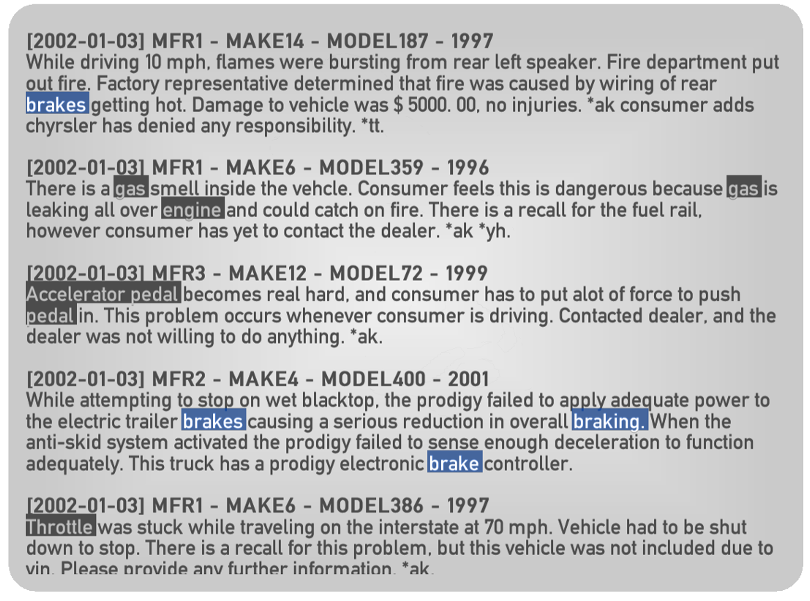
\includegraphics[width=\columnwidth]{document_small.png}
	 \caption[Document Widget]{The document viewer, the words highlighted in blue
	 are selected. The words highlighted in grey are the co-occurring entities}
	 \label{figure:document}
	\end{figure}
    % ===================

The document widget is toggle-based and is by default hidden from view. 
Once activated, an animation will expand its dimension from a single pixel to its full size at the
activation coordinate, a reverse animation is used to deactivate the panel. Once
fully visible, the document widget embed itself with two different interaction
regions. The left region, which takes up 80 percent of the panel, is used for
relocating the document widget to a different position. The right region is
designated for scrolling through the documents.





\section{Data Filters}
In this section, we describe the time and hierarchy widgets. These are used to
model the fixed fields (date, make, model, etc.) in the complaint documents.
They are domain specific and are used to filter data into logical
subsets. See Figure \ref{figure:filterFull} for a close up of our data
filters.

    % ===== Figure =====
	\begin{figure}
	 \centering  
	 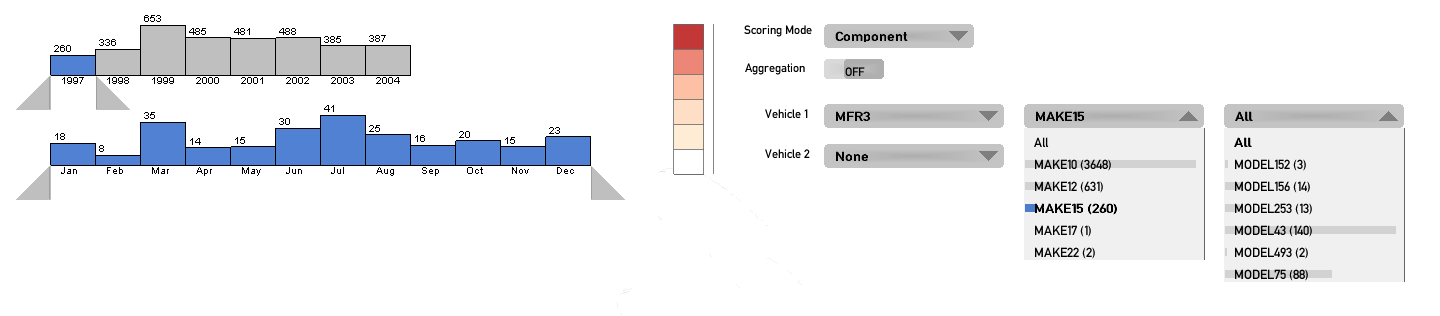
\includegraphics[width=\columnwidth]{filter_full.png}
	 \caption[Interactive Filters]{Time Slider Widget and Hierarchy Widget in
	 interactive mode}
	 \label{figure:filterFull}
	\end{figure}
    % ===================
    
 
    % ===== Figure =====
	\begin{figure}
	 \centering  
	 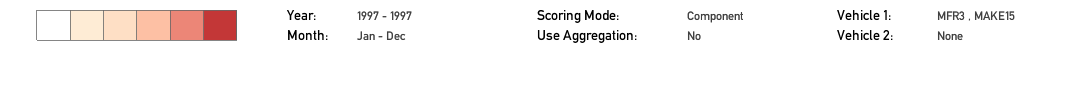
\includegraphics[width=\columnwidth]{filter_compact.png}
	 \caption[Compact Filters]{Time Slider Widget and Hierarchy Widget in compact
	 mode}
	 \label{figure:filterCompact}
	\end{figure}
    % ===================  
    
\subsection{Hierarchy Filter Widget}
The hierarchy widget is designed to model inclusive relationship, in particular,
it is specifically designed to address the need to for comparison (R2) and trend
finding (R3). For our problem domain, this relationship is represented as the
organizational hierarchy. Our data contains four such fields: manufacturer,
make, model and model year. For example: Civic (Make) belongs to Honda
(Manufacturer). These filters are shown as a variant of the combo boxes which
supports single selection, each item in the filter shows the name and the number
of documents associated with this organizational level. Rather than having the
readers comparing items by reading the numbers in text format, we double-encoded
the number of document as a horizontal histogram in similar style as the scented
widget approach in \cite{Willett2007}. The bar for each item in the widget is shaded
in light grey, and turns blue when the item is selected. 

Each level of the hierarchy is shown in individual filters. We position the
filters left-to-right across the display space, from the most general to most
specific classification. Each filter's content is 
dependent on the selection made on its parent. For example, the ``make''
selection widget will contain different makes if ``GM'' is the selected manufacturer than
it would for ``Chrysler''.  Non-top level hierarchy widgets remain hidden from view 
until it has selectable content, thus at the start, only the top level 
(manufacturer) filter widget is visible.




\subsection{Time Filter Widget}
The time dimension is encoded as a histogram, with the height of each bar denoting 
the volume of unique complaints for that time period. There are several granularity 
options with our document collection: daily, weekly, monthly or yearly. From an 
analysis of the incoming volume of documents, we found that daily and weekly 
granularity levels resulted in too much noise, these are discarded in favour
of months and years.

The widget is made up of two sliders. The top slider represents time
period in years, and the bottom slider represents time periods in months. 
Labels at the top of each bar give the numerical representation of the volume of
documents, note for the month slider the volume is the accumulated sum across
selected years. Makers at the bottom of each slider are used to select contiguous 
blocks. Selections of months and years are independent, for example, a person
can select January to June, between 2000 and 2005. This selection behaviour allows
people to focus and filter based on seasons and other sectional based divisions.

Interactions with the sliders are done through their markers as mentioned above, or directly
on the histogram bars. A double tap action on the year slider's bar provides a shortcut
to select the entire year. An animated transition is used to interpolate the
height of the histogram bars.



\subsection{Compact View}
The system provides a compact panel that encapsulates the legend, time and
hierarchy widgets as a work around to create more screen spaces for the main
visualization. As seen in Figure \ref{figure:filterCompact}, the compact view
removes much of the interactive GUI elements and replaces them with textual
summaries placed across the top of the display. It allows viewers to zoom in
closer and place interactive widgets in spatial positions that would have
otherwise cause occlusion issues. A swipe gesture is used to toggle between the 
two views.





%%%%%%%%%%%%%%%%%%%%%%%%%%%%%%%%%%%%%%%%%%%%%%%%%%%%%%%%%%%%%%%%%%%%%%%%%%%%%%%%
%\daniel{talk about waiting when making a selection}

\section{Design for Touch Surface}
Touch enabled system can be deployed in situations that are otherwise cumbersome
for systems that use mouse/keyboard input. For example, a
walk-up-and-use scenario in a public place or within a meeting in an office
setting. Our visualization is designed for these settings where traditional input devices may
not be available, in particular the visualization system is suited for large
displays. In this section we describe the gesture and interaction designs.


\subsection{Semantic Zones}
Zones are used to segment our display space and to process touch events. 
Each zone consists of one or more polygonal defined areas with
predefined semantics for handling touch based gestures. In the event that the zones overlap
each other and the system receives an event, the event will be propagated to the zone
with the highest priority, the remaining zones will ignore the event. The priorities are 
fixed and predetermined.

When a touch point is registered by the sensor hardware, the coordinate of the
touch point is checked to see which zone it is in, a coupling is created to
identify the touch point with a specific zone, the coupling will remain until
the touch point is removed. The reason for this approach is to allow higher error tolerance, we
want to avoid sudden changes of semantics which would defy user expectations.
This approach allows a subset of our dragging gestures (lens handle, slider
makers and scrolling) to continue to execute even if the actual touch point is
move off the predefined areas.

In the list below, we summarize the different zones in the system:
\begin{itemize}[noitemsep]
  \item Visualization Zone: The main visualization, handles selection
  and deselection semantics of \threed objects, as well as heatmap selection.
  \item Time Zone: Covers the year and month time sliders 
  \item Filter Zone: Covers the organizational hierarchy filters
  \item Lens Zone: Handles semantics for change the physical attributes of a
  lens widget
  \item Document Zone: Covers the document widget
  \item Empty Zone: An empty zone is specially designated zone that is none of
  the above. Empty zone handles gestures related to camera and miscellaneous
  functions.
\end{itemize}

The priority of the zones are in reversal usage order. The most data specific
widget, the document widget, has the highest priority, followed by lens, and the
visualization zone. The remaining ones have the same priority as they have
static positions.
 

\subsection{Gesture Design}
While we tried to adhere to commonly accepted gestures for navigation and
selection based tasks, our gesture design is also influenced heavily by the  
hardware and the perceived usage scenario: an infrared sensor overlay placed
atop a large, nearly vertical display screen. The hardware setup has several
design implications. The infrared sensor is imprecise because it senses
movements instead of real touches, as such it is possible to introduce
false positives due to hand posture and orientation. Software heuristics can be
used to mitigate the consequences of these untended noises, however,
there are ambiguous cases where software logic cannot guarantee the correct
outcome. For example, imagine a single handed gesture with the thumb and index
finger, we have noticed through experimental trials that the knuckles on the
other fingers are often picked up as extra touch points as well due to their
proximity to the sensor. In this case, it is difficult to tell which points
are intentional without additional information such as camera or depth image. 
As the sensor provides only the XY coordinates, we cannot infer hand orientations. Thus, we decided
to abandon any complex, explicitly-singled-handed, multi-fingered gestures in
favour of a simpler, less error prone approach.

The final gesture set is  an accumulation of several design iterations.
At each iteration, fellow lab members were asked to pilot-test the new gesture
recognitions and heuristics, their reactions and feedback were then incorporated 
into the next design iteration. 

Within the current iteration, there are two types of basic touch gesture semantics: 
a short-touch and a long-touch. A short-touch consists of any gesture
where the initial position is held for less than a threshold of 450 milliseconds, 
while a long-touch is the opposite. The threshold is derived from the pilots
studies.

Using the short-touches and long-touches as building blocks, we
constructed a more complex gesture set: 
\begin{itemize}[noitemsep]
  \item Touch/Tap: A short-touch followed by disengaging the gesture.
  \item Hold: A long-touch followed by disengaging the gesture. 
  \item Drag: A short-touch followed by some movement.
  \item Drag-Hold: A long-touch followed by some movement.
  \item Swipe: Swipe is a fast drag event.
\end{itemize}

Gestures are designed to be discrete and cannot be transitioned from one to 
another, for example, a dragging gesture to change the selected months cannot 
be transitioned to making a selection on the \threed visualization.

Below we summarize the system's interactions:
\begin{itemize} [noitemsep]
  \item Perspective Manipulation: Perspective manipulation consist of rotation
  of \threed model and camera zoom. Rotation is achieved with a
  single point horizontal or vertical drag gesture, which corresponds to
  rotation of the XZ and XY planes. Zooming events are triggered by bringing
  together two touch points closer together or further apart. All perspective
  manipulations must start in the empty zone.

  \item Entity Selection: Entity selection is triggered with a single touch.
  
  \item Tooltip: A hold gesture, or drag-hold gesture over the heatmap's cells will toggle the tooltip. 
  
  \item Lens Manipulation: A lens widget is created by specifying its diameter
  with two hold points, for example using index fingers on left and right hand
  to create the diameter. We impose a minimum and maximum diameter length to
  keep the physical size of the lens within reason, with our display hardware,
  we use the range between 100 to 500 pixels. Dragging gestures performed on the inner part
  of the lens shift the lens' location, while dragging gestures performed on the
  border resize the lens with respect to the point's distance away from the
  centre. A resize that results in a diameter that falls below the minimum
  threshold removes the lens widget all together. The handle tab on the
  widget adjusts the depth parameter, dragging the handle counter-clockwise
  increases the cutting depth, while the reverse decreases the cutting depth, we
  modelled this behaviour after the zooming mechanism on the barrels of camera
  lenses.
  
  \item Text Browsing: The document widget is toggled with a hold gesture over 
  the  empty zone. An active document widget has two zones, the left-most 80 percent
  of the document panel is used for reposition, while the right-most 20 percent for scrolling.
  Both  reposition and scroll actions use the drag gesture.

  \item Hierarchical Filters: A single touch gesture is used to open, close and to
  make selections. Scrolling is achieved by performing a vertical drag gesture on the item list.
  
  \item Time Sliders: Single touch gesture is used to send select events to
  individual time sliders. Dragging gesture is used to move the slider markers.
\end{itemize}

    % === Figure ===
	\begin{figure}
	 \centering  
	 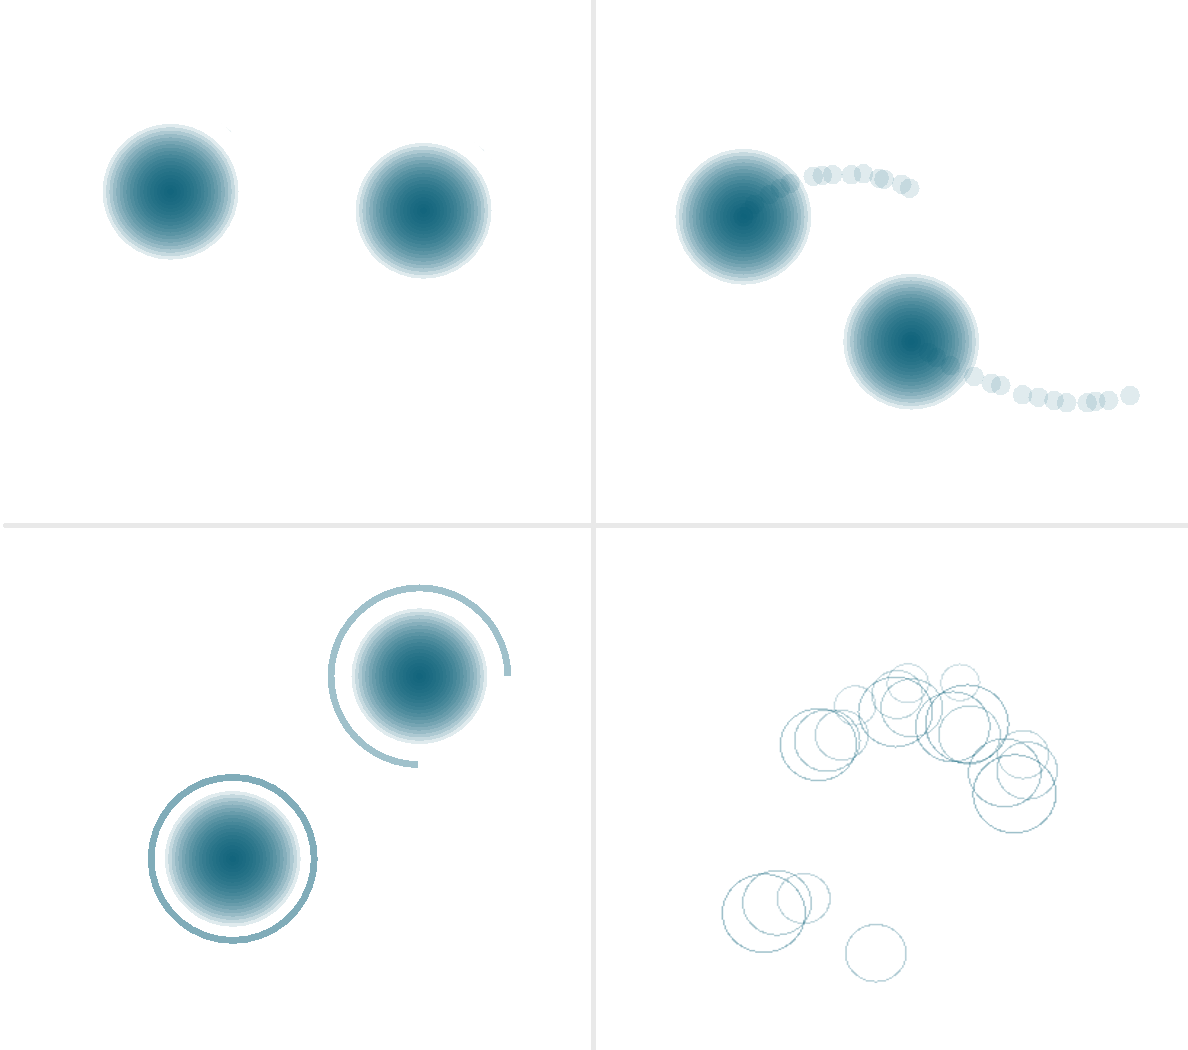
\includegraphics[width=\columnwidth]{feedback.png}
	 \caption[Visual Feedback]{Clockwise from top left: short touches, transitions,
	 unrecognized points, long touches.}
	 \label{figure:feedback}
	\end{figure}
	% =============== 
 

\subsection{Visual Feedback}
When using the keyboard, mouse and other hardware peripherals, actions are
rewarded with some type of haptic feedback, for example we know when a key on a 
keyboard is pressed of depressed. This behaviour allows people to be more keenly 
aware of the system's current state. This is not true with touch interfaces,
with touch and sensing technology, it is possible for touch points to become lost during a gesture, 
this is due to the users unconsciously lifting their fingers. When this happens people 
can get confused because they may be not be aware that their touch points are lost 
since their fingers are still contacting the surface, there are no feedback
system to alert the actual touch point had disappeared. To accommodate the lack of
physical responses, we implemented our own visual feedback. We created
four different types of visual cues, which we summarize below and can be seen in
Figure \ref{figure:feedback}. 

\begin{itemize}[noitemsep]
  \item Short Touch Point: Whenever a touch point is registered, we render a gradient
  circle at the XY screen coordinate as detected by the sensor. The
  radius of the circle is slightly larger than the average fingertip such that
  is is always visible, this is about 15 pixels on our display. The position of
  the circle is updated to synchronize with sensor updates, and is removed
  when the touch point is rescinded. This visual cue gives viewers immediate
  feedback of the active touch points.

  \item Long Touch Point: A long touch point has the same basic visual cue as a short touch point.
  A long touch starts off as a short touch point, a ticking timer running in the
  background determines when the short touch transitions into a long touch. We
  visualize this timing sequence as an arc outside of the circle, the arc grows
  with an increasing central angle and opacity that are mapped to the amount of
  time elapsed. A long touch gesture is achieved once the arc has travelled
  the entire circumference, becomes a ring and locks down. Any interruption
  during the transition phase will remove the animation, the gesture will return
  back to a normal touch point.

  \item Trails: The system keeps track of previous updates for all points.
  We visualize up to the last 10 most recent updates as breadcrumb trails. 
  The trails serve as a reminder of what type of high level gesture is being
  performed, furthermore it serves as additional visual cue to identify the
  current touch point location. The trail points are rendered as smaller
  versions of touch points.
   
  \item Removals: These visual cues are used to denote any removals sensed by
  the hardware device, these includes the active points sensed by our software
  and also any other ones that were rejected by our evaluating heuristics. This
  cue gives the viewers some sense of the hardware capabilities and
  deficiencies. We think this is useful as a learning device, viewers are able
  to see where they may inadvertently cause unwanted touch points and use this
  experience to adjust how they operate their gestures next time they interact
  with the display. We visualize this as unfilled circles that decrease in
  opacity and radius with time, they are removed from the system when the radius
  reaches zero.
\end{itemize}
 
An additional visual feedback was created to visualize processing time. Due the 
size of dataset, the system may incur a slight delay between re-evaluation of the
visualization. We draw a small clock icon at the position where the last action 
was performed to indicate the system is processing, the clock fades into the back
ground once the data processing is completed. 





